\section{Introduction}
Introduction

\newpage

\section{My first section}
\label{section:Introduction}
To describe methods of CI with NodeJS

\subsection{Introduction to Agile Development and the Role of Development Operations in Modern Web Applications}

% \begin{figure}[h!]
%   \centering
%       
\includegraphics[width=0.4\textwidth]{images/Perlin-Coherent.png}
%   \caption{Just some example figure}
% \end{figure}

\subsection{The Foundations of Continuous Integration and Automatization in Development Operations}
\subsection{Development and Deployment with MEAN}
\subsection{Test Driven Development with MEAN}
\subsection{Containerization and Deployment with Docker}
\subsection{Building Continuous Integrations and Deployment with NodeJS}


% \subparagraph{subparagraph}
% \footcite{meyer2014continuous}
%
% \begin{itemize}
%   \item Itemlist 1
%   \item Itemlist 2
% \end{itemize} \cite{cranorplatform}
%
% \section{Next Section}
% \label{section:Label}
%
% \textit{Texit Option}
%
% \begin{figure}[h!]
%   \centering
%       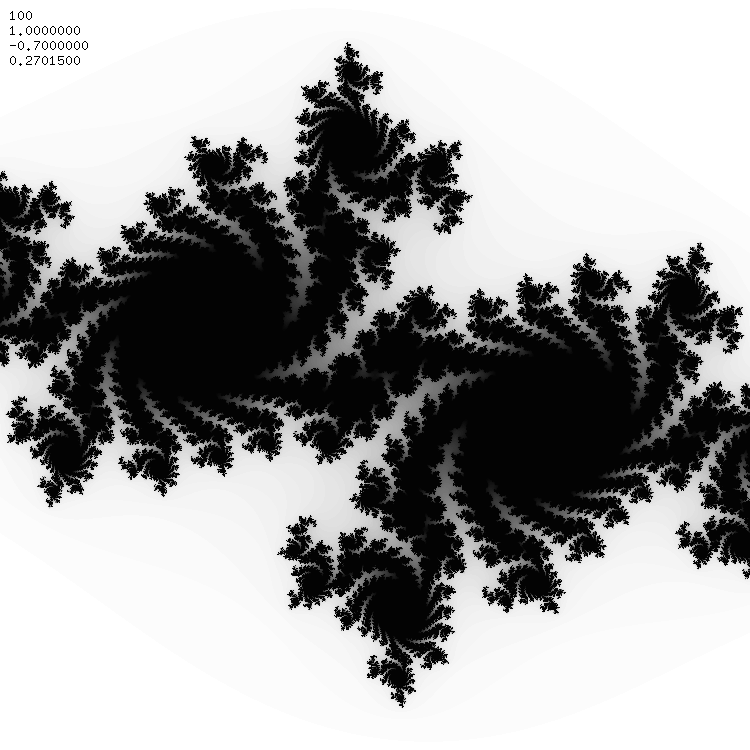
\includegraphics[width=0.2\textwidth]{images/Julia-Fractal.png}
%   \caption{Exampelimage}
% \end{figure}
%
% \subparagraph{Unforgeability}
% \label{subp:subparagraph_name}
%
% Graphic by \url{http://en.wikipedia.org/wiki/Pretty_Good_Privacy#/media/File:PGP_diagram.svg}
